
Dada la siguiente topología:

\begin{itemize}
  \item La máquina uml1 realiza un anuncio de prefijos, y es la única
  autorizada
  \item La máquina uml3 también intentará hacerlo, pero OpenFlow lo impedirá
\end{itemize}

\begin{figure}[h]
  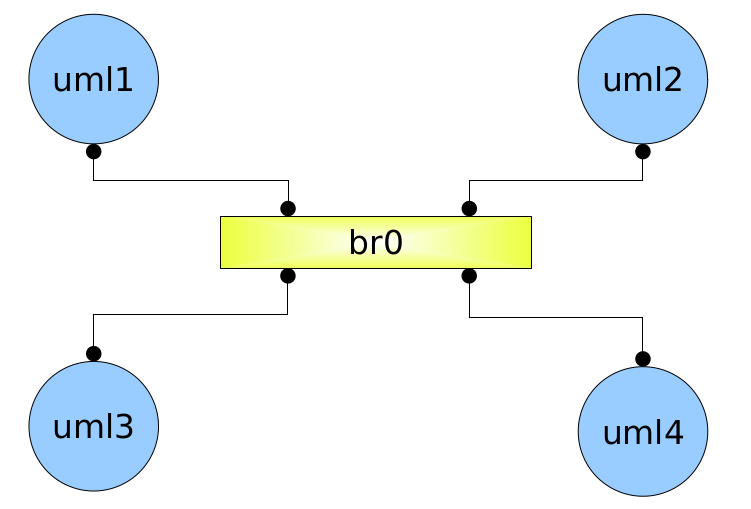
\includegraphics[width=\textwidth]{ovs-ofctl.png}
  \centering
\end{figure}

Anuncios de prefijos:

\begin{itemize}
  \item uml1: 2001:db8:1::/64
  \item uml3: 2001:db8:3::/64
\end{itemize}

\begin{minted}{bash}
  # net.conf
  defsw br0 uml1.0 uml2.0 uml3.0 uml4.0
\end{minted}


